% vim: ft=tex
\chapter{Project monitoring}
\section{Performance analysis}
\subsection{Weekly overview}

\autoref{fig:projmon:weekly} illustrates the weekly time spent on this bachelor
thesis. The thick horizontal line represents the planned effort of 28.5 hours a
week, which has been calculated using the risk analysis explained
in~\autoref{sec:projplan:est-time}.  Milestones are denoted by the green
labels. The legend along the x-axis represents the semester weeks, including
the particular RUP phases.


\begin{figure}[]
	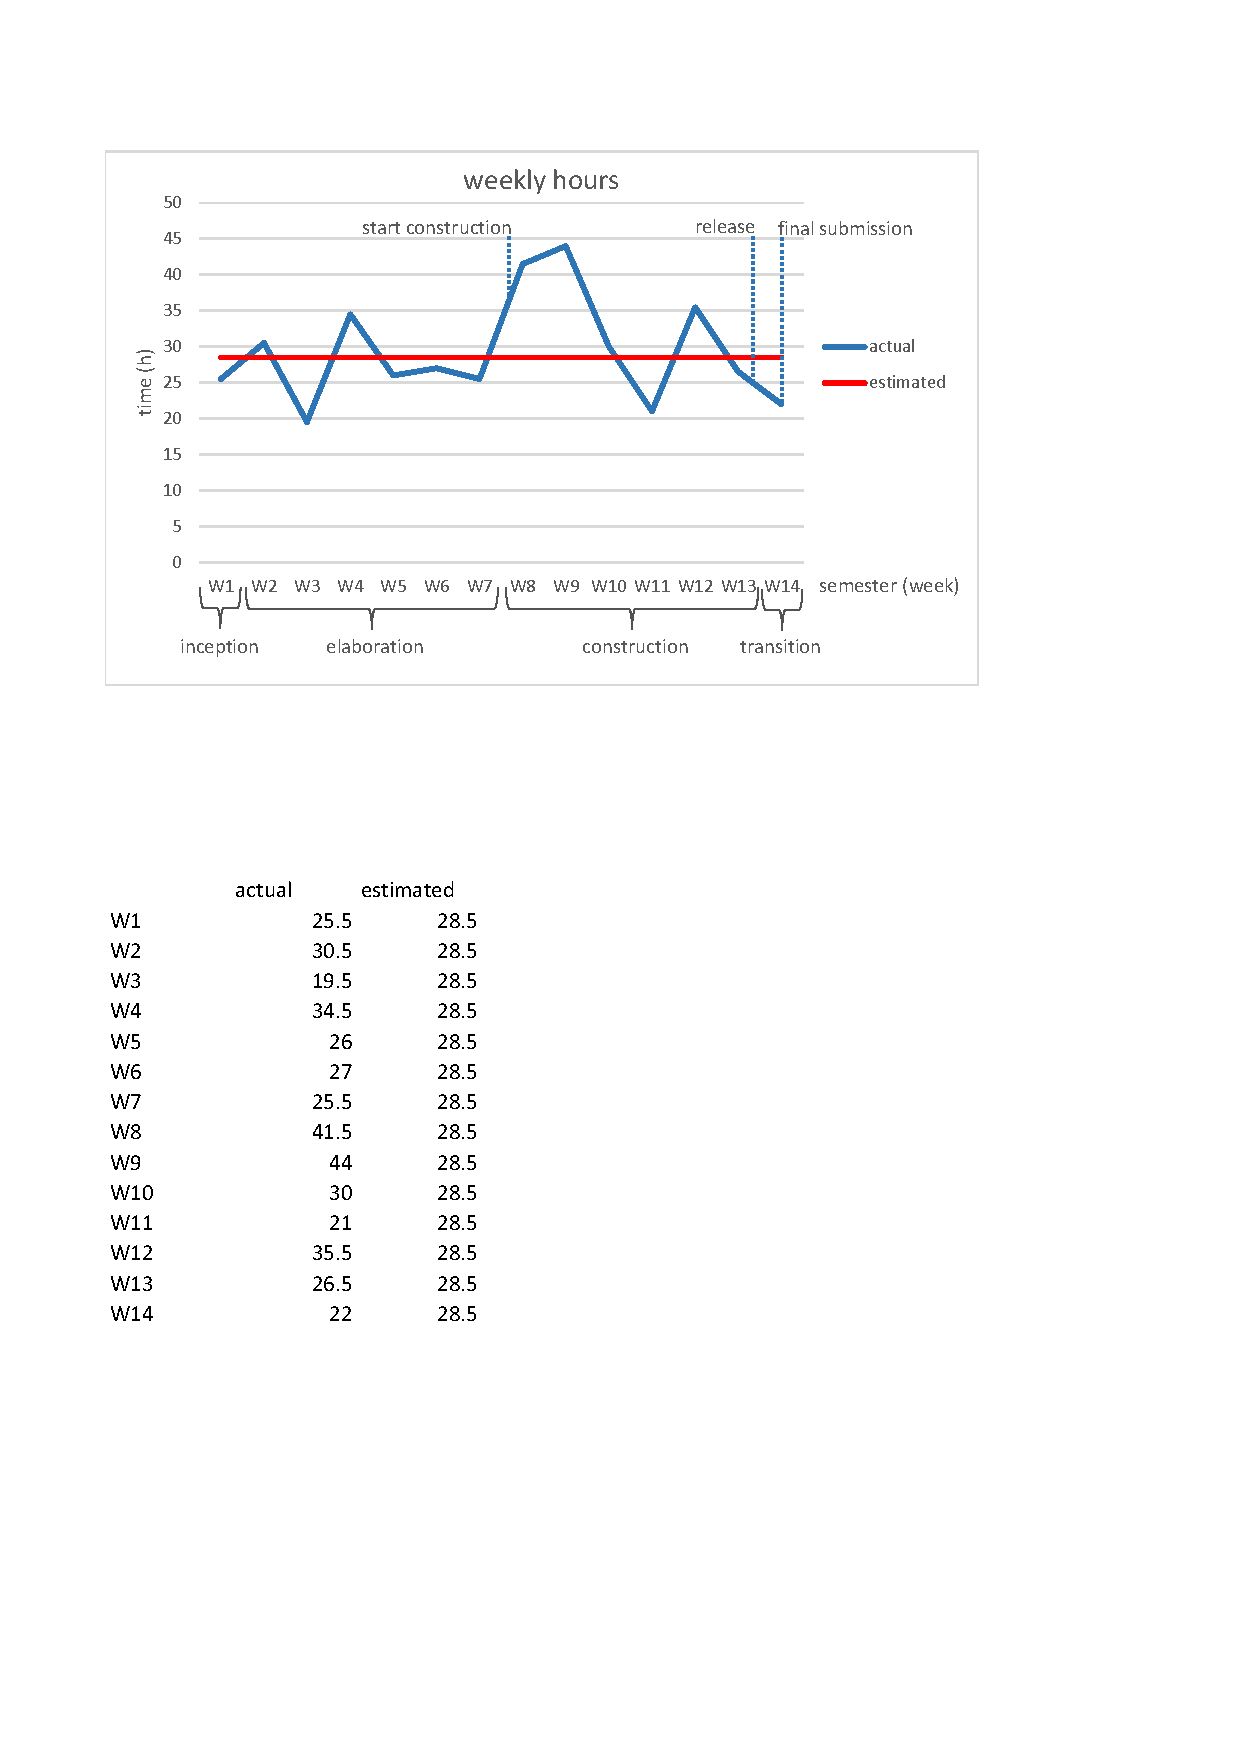
\includegraphics[trim=2cm 18.3cm 4.6cm 2.8cm, clip=true, width=\textwidth]{img/project_monitoring_weekly_diagram.pdf}
	\caption{weekly hours}
	\label{fig:weekly:hours}
\end{figure}

% TODO Translate
Wie man aus dieser Grafik herauslesen kann, haben wir zu Beginn der Arbeit 
am wenigsten Stunden pro Woche aufgewendet. Das liegt daran, dass wir zuerst die 
genauen Anforderungen abklären mussten und teilweise erst nach einer Besprechung 
oder einer Rückmeldung an bestimmten Punkten weiterarbeiten konnten. 
Vor dem Meilenstein „Release“ hatten wir alle Informationen zusammen und 
konnten mit vollem Elan die Anforderungen umsetzen.


\begin{table}[H]
  \centering
  \begin{tabular}{|p{100mm}|p{35mm}|}
    \hline 	\bf Planned HSR hours & 720h \\ \hline
	\bf Estimated hours & 816h \\ \hline
	\bf P. Wenger worked hours & 413h \\ \hline
	\bf M. Schuler worked hours & 403h \\ \hline
	\bf Everhour tags & 14 \\ \hline
	\bf Github issues & 94 \\ \hline
	\bf Github tasks & 230 \\ \hline
	\bf Biggest issue \#33 Refine Document & 80h \\ \hline
  \end{tabular} \\
  \caption{project stats}
  \label{tab:projectstats}
\end{table}


% TODO translate
Die von der Modulbeschreibung geforderten, Soll-Stunden wurden um 10% überschritten haben. 
Der Grund der Überschreitung ist unteranderem
die Implementation der optionalen Features und die grossflächig angelegten Tests.
Die einzelnen Personen haben ein sehr ausgeglichenes Stundentotal. 
Das liegt daran, dass wir in regelmässigen Abständen eine Auswertung 
in Everhour gemacht haben und dadurch die Tasks gerechter verteilen konnten. 

\begin{figure}[]
	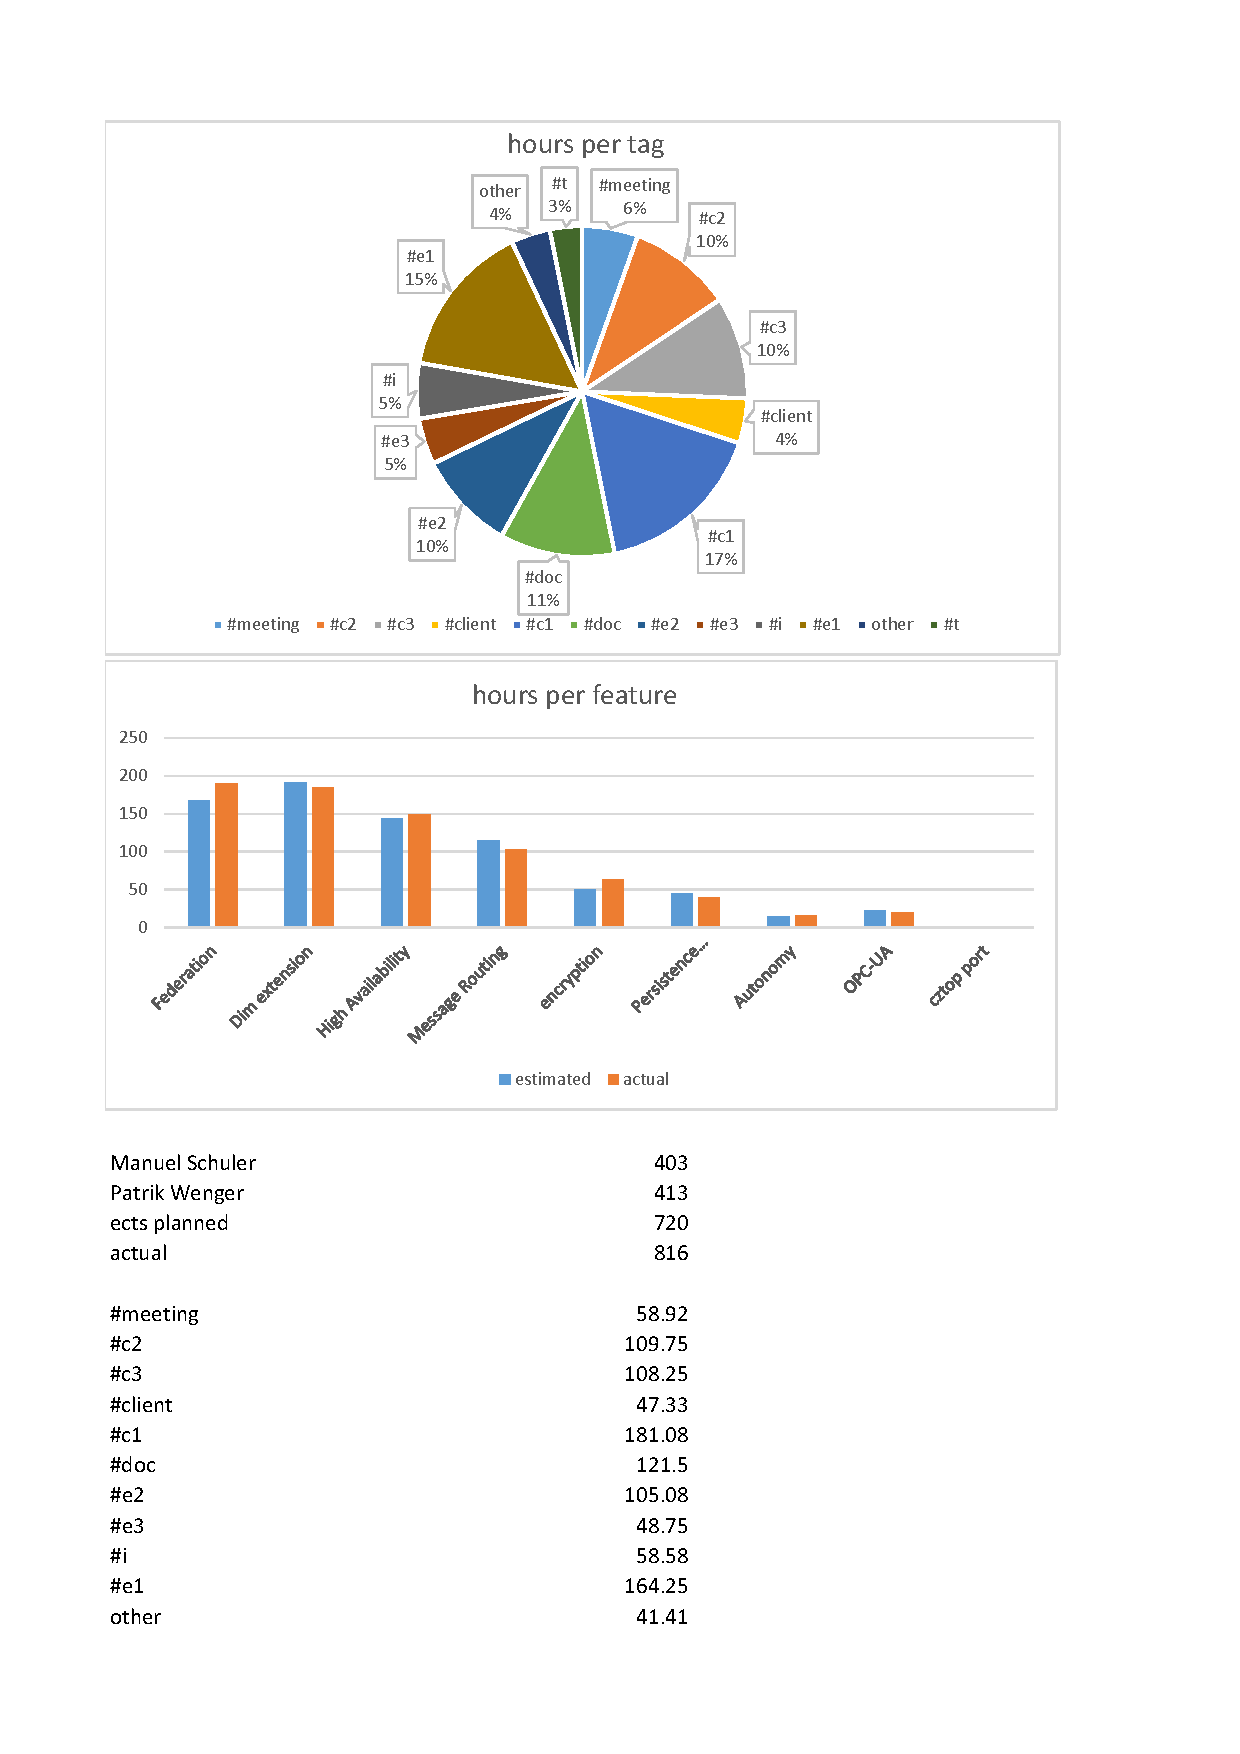
\includegraphics[trim=4cm 18.8cm 3.5cm 2.8cm, clip=true, width=\textwidth]{img/project_monitoring_diagrams.pdf}
	\caption{hours per tag}
	\label{fig:hours:per:tag}
\end{figure}

8\% der ganzen Projektdauer wurde für Projektmanagement
und Meetings aufgewendet. 2\% davon sind für Requirements besprechung mit dem Kunden. Die Verteilung
entspricht vollumfänglich der geplanten Phasen. Es gibt kein \#Tag welches speziell heraussticht. 


\subsection{Aufgewendete Stunden nach Feature}
% TODO Translate
Da wir in dieser Arbeit ein bestehendes Produkt erweitert haben war es zu beginn an
schwierig die Aufwände abzuschätzen. Die Soll/Ist Abschätzungen wurden von Iteration zu Iteration
immer genauer. Nachfolgend die Soll/Ist Aufwandschätzung der einzelnen Feature.

% TODO checklist item: each up to 4h

\begin{figure}[]
	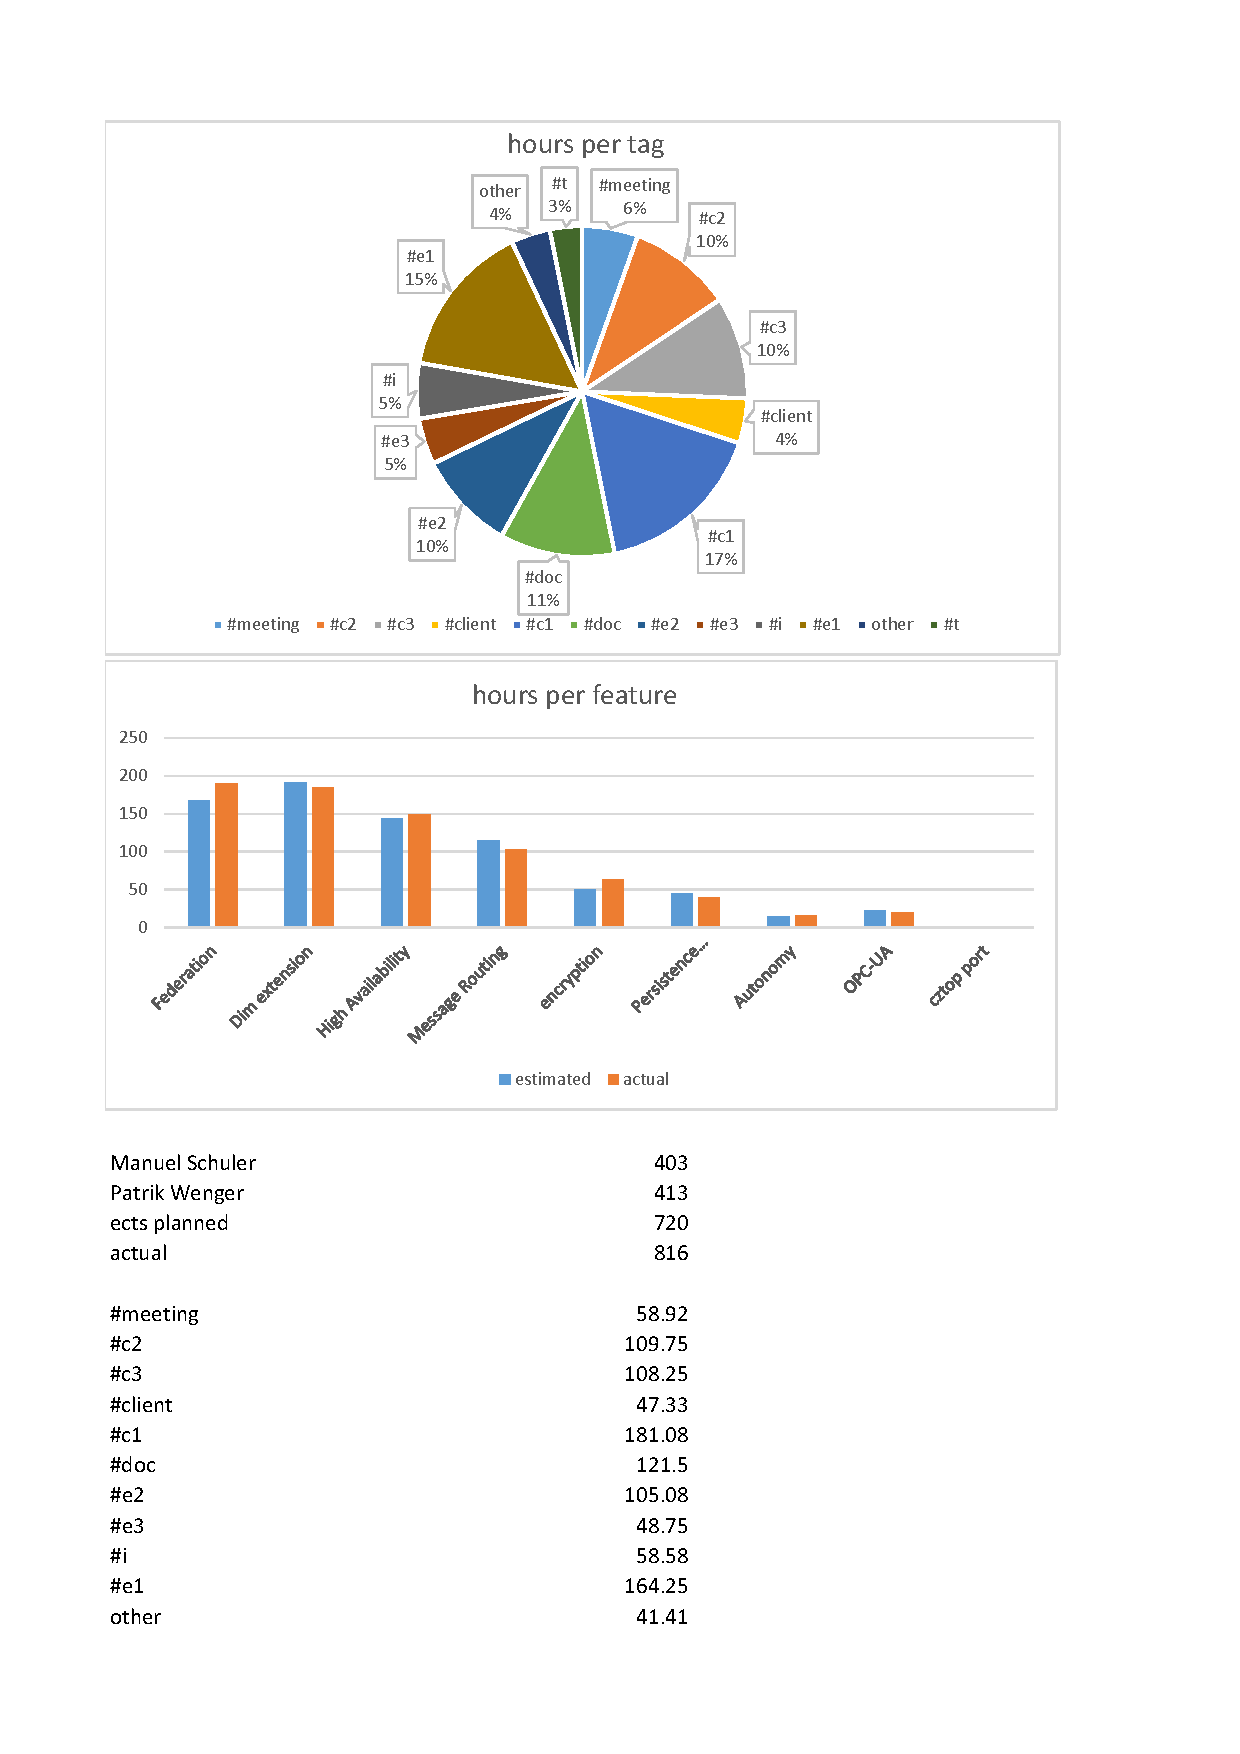
\includegraphics[trim=2cm 11cm 3.5cm 11.5cm, clip=true, width=\textwidth]{img/project_monitoring_diagrams.pdf}
	\caption{hours per feature}
	\label{fig:hours:per:feature}
\end{figure}

% TODO translate
Die ersten Feature brauchten knapp mehr Zeit als geplant. Es wurde schon früh während der Prototyp Phase
gemerkt das es mehr Zeit braucht als geplant in die Einarbeitung in Roadster. Das fehlende Wissen und
die "Perfektionswut" waren unteranderem Grund dafür.
Im weiteren Projektverlauf konnte die Performance der einzelnen Projektmitarbeiter gesteigert werden
was auf das erlernte Wissen über Roadster zurückzuführen war, sowie durch die gut
Strukturiere Architektur von Roadster was uns das Erweitern der Software sichtlich erleichtert hat.


% TODO translate
Die Archivdaten unseres Everhour Projekts befinden sich auf dem Moodle. 
In diesem kann detailliert nachverfolgt werden, 
für welche Tasks wir wie viel Zeit aufgewendet haben.

\subsection{Effort by activity}
% TODO category diagram
